

\documentclass{beamer}
\usepackage{listings}
\usepackage{amsfonts}
\usepackage{dsfont}
\usepackage{amsmath}
\usepackage{bbm}
\usepackage{verbatim}
\usepackage{listings}
%\usepackage{tipa}
\usepackage{tikz}
\usetikzlibrary{fit}
\usepackage{color}
\usepackage{booktabs}
\usepackage{tipa}
\usepackage{amssymb}
\usepackage{verbatim}
\usepackage[absolute,overlay]{textpos}
\usepackage{pifont}% http://ctan.org/pkg/pifont
\newcommand{\cmark}{\ding{51}}%
\newcommand{\xmark}{\ding{55}}%
\usetikzlibrary{bayesnet}
\usetikzlibrary{decorations.markings}
\usetikzlibrary{decorations.pathmorphing}
\tikzset{squiggle/.style={decorate, decoration={snake,amplitude=.4mm}}}
\usepackage{xcolor}
\definecolor{pop1}{HTML}{1F78b4}
\definecolor{pop2}{HTML}{164C13}
\definecolor{pop3}{HTML}{d95F02}
\definecolor{orange}{HTML}{d95F02}
\definecolor{teal}{HTML}{1b9e77}
\newcommand{\pop}[1]{\textcolor{pop1}{#1}}
\newcommand{\popp}[1]{\textcolor{pop2}{#1}}
\newcommand{\tree}[1]{\textcolor{pop3}{#1}}
\newcommand{\orange}[1]{\textcolor{orange}{#1}}
\newcommand{\teal}[1]{\textcolor{teal}{#1}}


\newcommand{\nextForm}[1]{\rotatebox[origin=c]{270}{$_{\curvearrowright}$}$_{#1}$}
 
\usepackage{amsfonts}
\usepackage{tabularx}
%\usepackage{color}
\usepackage{graphicx}
\usepackage{booktabs}
\usepackage{xcolor}
\usepackage{tikz}
\usetikzlibrary{trees}
\usetikzlibrary{fit}
\usetikzlibrary{calc}
\usetikzlibrary{bayesnet}
\usepackage[absolute,overlay]{textpos}
\usepackage{stmaryrd}
\newcommand{\sem}[1]{\llbracket #1\rrbracket}
\newcommand{\tuple}[1]{\ensuremath{\left \langle #1\right \rangle}}
\usepackage{booktabs}
\usepackage{tipa}
\usepackage{amssymb}
\usepackage{verbatim}
\usepackage[absolute,overlay]{textpos}
\usepackage{pifont}% http://ctan.org/pkg/pifont
\newcommand{\cmark}{\ding{51}}%
\newcommand{\xmark}{\ding{55}}%
\usetikzlibrary{bayesnet}
\usetikzlibrary{decorations.markings}


\usepackage[utf8]{inputenc}

\usepackage{amssymb}% http://ctan.org/pkg/amssymb
\usepackage{pifont}% http://ctan.org/pkg/pifont

\usepackage{fancyvrb}

%% Program ::=
%%   (if Bool List
%%     (append RecursiveList
%%             RecursiveList
%%             RecursiveList))
%% RecursiveList ::= List
%%          | (recurse List)

            
\begin{SaveVerbatim}[]{ListSketch}
Bool ::= (<= Int) | (>= Int)
       | (= Int)
Int  ::= 0
       | (+1 Int) | (-1 Int)
       | (length List)
       | (head List)
List ::= nil | X
       | (filter Bool List)
       | (tail List)
       | (list Int)
\end{SaveVerbatim}

\begin{SaveVerbatim}[]{ListSketchFull}
Program ::= (if (Bool Int)
                List
                (append RecursiveList
                        RecursiveList
                        RecursiveList))
RecursiveList ::= List
                | (recurse List)
Bool ::= (<= Int) | (>= Int)
       | (= Int)
Int  ::= 0
       | (+1 Int) | (-1 Int)
       | (length List)
       | (head List)
List ::= nil | X
       | (filter Bool List)
       | (tail List)
       | (list Int)
\end{SaveVerbatim}

\begin{SaveVerbatim}[]{Reverse}
(if (<= (+1 0) (length X))
    X
    (append (recurse (tail X))
            (list (head X))))
\end{SaveVerbatim}
\begin{SaveVerbatim}[]{Reversep}
(if (= (+1 0) (length X))
    X
    (append (recurse (filter (<= (+1 0)) (tail X)))
            (list (head X))))
\end{SaveVerbatim}

\begin{SaveVerbatim}[]{Count}
(length (filter (= (head X)) (tail X)))
\end{SaveVerbatim}

\begin{SaveVerbatim}[]{Countp}
(-1 (length (filter (= (head X)) X)))
\end{SaveVerbatim}

\begin{SaveVerbatim}[]{Sort}
(if (<= (+1 0) (length X))
    X
    (append (recurse (filter (<= (head X)) (tail X)))
            (list (head X))
            (recurse (filter (>= (head X)) (tail X)))))
\end{SaveVerbatim}

\begin{SaveVerbatim}[]{Sortp}
(if (= (+1 0) (length X))
    X
    (append (recurse (tail X))
            (list (length X))))
\end{SaveVerbatim}

\begin{SaveVerbatim}[]{TextSketch}
Program ::= Term
          | Program + Term
Term    ::= String
          | substr(Pos,Pos)
Pos     ::= Number
          | pos(Str,Str,Num)
Num     ::= 0 | 1 | 2 | ... 
          | -1 | -2 | ...
Str     ::= Character 
          | Character + String
Character ::= a | b | c | ...
\end{SaveVerbatim}

\newcommand{\theSystem}{\textsc{ProgramSample}}
\usepackage{arydshln}

\newcommand{\Expect}{\mathds{E}} %{{\rm I\kern-.3em E}}
\newcommand{\Probability}{\mathds{P}} %{{\rm I\kern-.3em P}}

\DeclareMathOperator*{\argmax}{arg\,max}
%Information to be included in the title page:
\title{Growing libraries of concepts with wake-sleep program induction}
\author{Kevin Ellis \& Mathias Sabl\'e Meyer\\Joint work with: Lucas Morales, Armando Solar-Lezama, Joshua B. Tenenbaum\\Heavy inspiration from: Eyal Dechter}
\institute{MIT} 
%\date{November 2017}
  
 
\begin{document}
 
\frame{\titlepage}

\begin{frame}{The Language of Thought}
\begin{tikzpicture}
    \node at (-3,1) {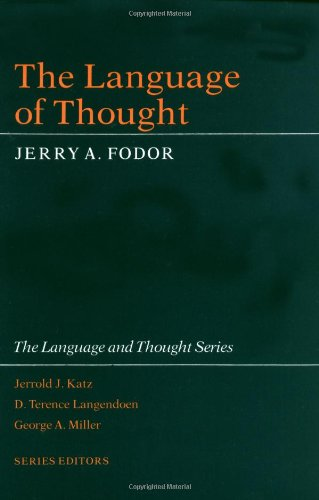
\includegraphics[width = 6cm]{Fodor.jpg}};
  \node at (2,2) {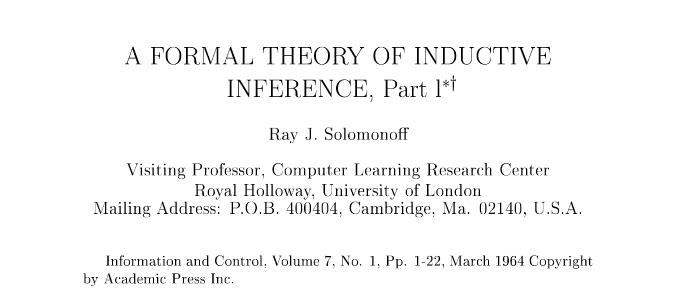
\includegraphics[width = 8cm]{Solomon.png}};
%
    \end{tikzpicture}
\end{frame}

\begin{frame}{Engineering the language of thought}
 \begin{tikzpicture}
    \node () {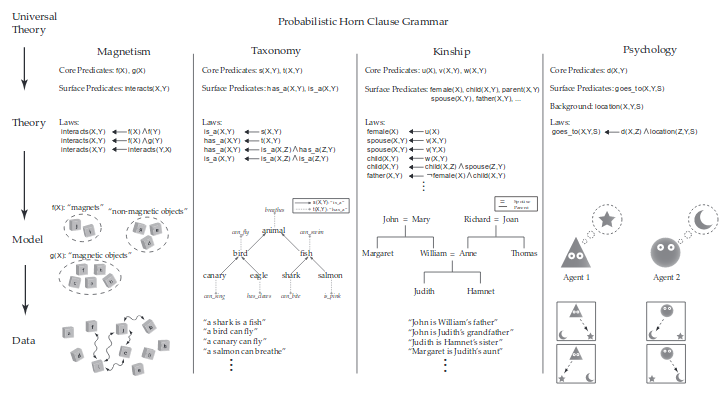
\includegraphics[width = 15.6cm]{theory.png}};
    \node at (-5,-4) {  Ullman et al 2012};
    \end{tikzpicture}
\end{frame}

\begin{frame}{Engineering the language of thought}
  \begin{tikzpicture}
    \node at(0,0) {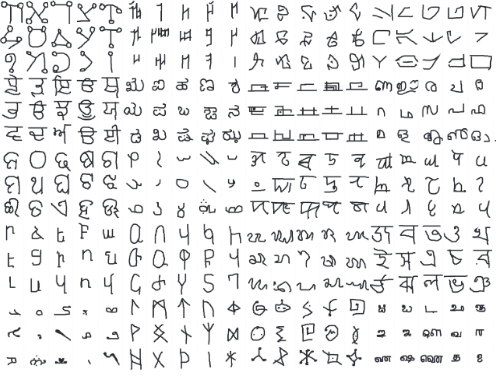
\includegraphics[width = 8cm]{characters.png}};
    \node at(-3,2) {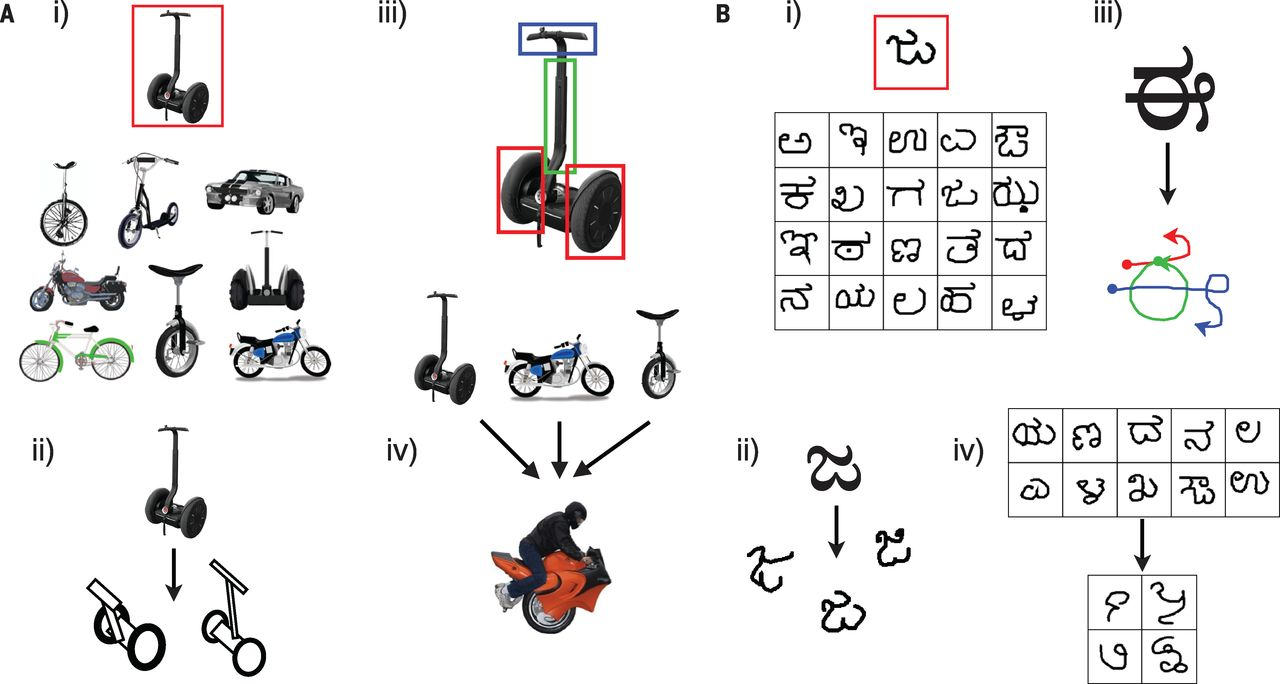
\includegraphics[width = 8cm]{Brendan.jpg}};

    \node at (-5,-4) {  Lake et al 2015};
    \end{tikzpicture}
\end{frame}



\begin{frame}{Growing a domain-specific language of thought}
  
  %  \Large
  Goal: acquire domain-specific knowledge needed to induce a class of programs


  
  \pause
  \vspace{1cm}

  \begin{itemize}
  \item Library of concepts (declarative knowledge)
    \item Search strategy (procedural knowledge)
    \end{itemize}
\end{frame}

\begin{frame}{DSL: Library of concepts}
\includegraphics[width = 11cm]{3DSL.png}
\end{frame}

\begin{frame}{DSL learning as Bayesian inference}
  \centering
  \begin{tikzpicture}
    \node[latent,align=center] (g) {DSL: \\concept library};
    \node[latent,below = of g,xshift = -2cm] (e1) {$\text{program}_1$};
    \node[latent,below = of g,xshift = 0cm] (e2) {$\text{program}_2$};
 \node[latent,below = of g,xshift = 2cm] (e3) {$\text{program}_3$};
    \node[obs,below = of e1] (x1) {$\text{task}_1$};
    \node[obs,below = of e2] (x2) {$\text{task}_2$};
    \node[obs,below = of e3] (x3) {$\text{task}_3$};
    \edge {g} {e1,e2,e3};
    \edge {e1} {x1};
    \edge {e2} {x2};
    \edge {e3} {x3};
  \end{tikzpicture}

\textbf{[Dechter et al., 2013]}  [Liang et al, 2010]; [Lake et al, 2015]

  \end{frame}

\begin{frame}{Amortized program inference}

  
  \includegraphics[width = 9cm]{rm.png}

  \begin{itemize}
  \item $\mathcal{D}$: DSL
  \item $p_n$: program
  \item $x_n$: task
  \item $Q$: Recognition model
    \end{itemize}

\end{frame}

\begin{frame}{DreamCoder}
  \begin{itemize}
  \item   \textbf{Wake:} Solve problems by writing programs
  \item \textbf{Sleep:} Improve DSL and neural recognition model:
    \begin{itemize}
    \item \textbf{Sleep-G:} Improve DSL (\textbf{G}enerative model)
      \item \textbf{Sleep-R:} Improve \textbf{R}ecognition model
      \end{itemize}
  \end{itemize}
  Based on Exploration-Compression algorithm by Eyal Dechter

\pause
  \vspace{1cm}
  
  \centering\begin{tikzpicture}
    \begin{scope}[shift = {(1,-1)}]
    \node[align = center](synthesis) at (6,4) {Search for \\programs: $p$};
    \node[align = center](DSL) at (3,1) {DSL: $\mathcal{D}$};
    \node[align = center](recognitionModel) at (9,1) {Recognition \\model: $q$};

    \draw [->,thick] (synthesis.-120) to[out = -150,in = 60] node[below,rotate = 45,align = center]{{\footnotesize Trains}\\{\footnotesize (Sleep-G)}} (DSL.30);
    \draw [->,thick] (synthesis.-60) to[out = -30,in = 120] node[below,rotate=-45,align = center]{{\footnotesize Trains}\\{\footnotesize (Sleep-R)}} (recognitionModel.150);
    \draw [->,thick] (DSL.east) to[out = -30,in = 210] node[above, align = center]{{\footnotesize Trains}\\{\footnotesize (Sleep-R)}} (recognitionModel.west);

    \draw [->,thick,dashed] (DSL.north) to[out = 90,in = 180] node[fill=white,align = center]{  \footnotesize{Inductive bias}\\\footnotesize{(Wake)}} (synthesis.west);
    \draw [->,thick,dashed] (recognitionModel.north) to[out = 90,in = 0] node[fill=white,align = center]{{\footnotesize Makes tractable}\\{\footnotesize (Wake)}} (synthesis.east);
  \end{scope}
    \end{tikzpicture}

\end{frame}

\begin{frame}{Wake phase}
  \centering\begin{tikzpicture}[scale=1.3]
    \node at (0,0) (d){DSL};
    \node at ([yshift = -2cm]d) (t){$\text{Task}$};

    \node at ([xshift = 2cm]t) (nn){
      \begin{tikzpicture}[x=2.5cm,y=1.25cm,transform canvas={scale=0.2,shift={+(-1,2.5)}}]
        \tikzstyle{neuron}=[circle,fill=blue!50,minimum size=20pt]
        \fill[fill=white] (-0.25,-0.5) rectangle (2.25,-4.5);
        \node[rectangle] at (1,1) {};
        \foreach \name / \y in {1,...,4}
            \node[neuron] (I-\name) at (0,-\y) {};
        \foreach \name / \y in {1,...,3}
            \node[neuron] (H-\name) at (1,-\y-0.5) {};
        \foreach \name / \y in {1,...,4}
            \node[neuron] (O-\name) at (2,-\y) {};
        \foreach \source in {1,...,4}
            \foreach \dest in {1,...,3}
                \draw [-latex] (I-\source) -- (H-\dest);
        \foreach \source in {1,...,3}
            \foreach \dest in {1,...,4}
                \draw [-latex] (H-\source) -- (O-\dest);
      \end{tikzpicture}
    };
    \node[align = center, text width = 1cm] at ([yshift = 0.6cm]nn.north) {\baselineskip=0pt \small Recognition model\par};
    \draw [->] (t.east) -- ([xshift = -0.5cm]nn.west);

    \node[draw,rounded corners, inner sep = 10] at ([xshift = 4.2cm,yshift = -1cm]) (s){Search};
    \node at ([xshift=-7pt,yshift=5pt]s.north west) {$\mathcal{D}$};

    \draw [->] ([xshift = 0.5cm]nn.east) -- ([yshift = -0.25cm]s.west);
    \draw [->,rounded corners] (d.east) -- ([yshift = 2cm]nn.center) -- ([yshift = 0.25cm]s.west);

    \node[align=left] at (7,-1) (f) {Frontier\\{\small (set of programs)}};
    \draw [->  ] (s.east) -- (f.west);

    \draw [->  ,rounded corners] (t.south) -- ([yshift = -0.5cm]t.south) -- ([yshift = -0.5cm] s.south |- t.south) -- (s.south);
    \node at ([xshift = 0.5cm,yshift = -0.75cm]s.south) {Spec};

    \node at (4,-3.5) {\textbf{\textsc{Wake: Problem Solving}}};
    
    
  \end{tikzpicture}

\end{frame}

\begin{frame}{Sleep-G Phase}
  Fragment grammar (\textbf{O'Donnell 2015})
  \vspace{1cm}
  
  \centering\begin{tikzpicture}
    \node at (0,0) (f1){Frontier$_1$};
    \node at ([yshift = -1cm]f1.south) (f2){Frontier$_2$};
    \node at ([yshift = -0.7cm]f2.south) (ff){\textbf{$\vdots$}};
    \node at ([yshift = -1.2cm]f2.south) (ff){\textbf{$\vdots$}};
    \node at ([yshift = -1cm]ff.south) (f3){Frontier$_N$};

    \node(c)[rectangle, rounded corners, draw, minimum width = 3cm, minimum height = 6cm, anchor = north west] at (2,1) {};
    \node[anchor=north] at (c.north) {Compression};

    \draw [-> ] (f1.east) -- (c.west|-f1.east);
    \draw [-> ] (f2.east) -- (c.west|-f2.east);
    \draw [-> ] (f3.east) -- (c.west|-f3.east);

    \node[right](d) at ([xshift = 1.2cm,yshift = 0.7cm]c.east) {DSL $\mathcal{D}$};
    \node[right](t) at ([xshift = 1.2cm,yshift = -0.7cm]c.east) {Weights $\theta$};
    \draw [-> ] (c.east) -- (d.west);
    \draw [-> ] (c.east) -- (t.west);

    \node at (c.center) {
\begin{tikzpicture}[scale=0.7]
    %% \node[rotate=30] at (-2,0) {\begin{tabular}{c}
    %%     \footnotesize Program:\\
    %%     \code{($\lambda$ (x) (+ (- x) 1))}
    %% \end{tabular}};
    %\node at (,0.5) {\code{cons}};
%    \node [rotate=90] at (-2.3,-0.5) {\small program};
    
          \node(l1) at (0,0) {};
  \node[color=pop3](p1) at (-1,-1) {\code{+}};
  \node[color=pop3](n1) at (0.7,-0.9) {\code{1}};
  \node(x1) at (0,-1) {\code{1}};
  \draw[color=pop3] (l1.south) -- (p1.north);
  \draw[color=pop3] (l1.south) -- (n1.north);
  \draw[color=pop3] (-0.5,-0.45) -- (x1.north);

  \node(t) at (-0.5,0.5) {};
  \draw (l1.south) -- (t.south);
  \node(c) at (-1.5,-0.2) {\code{cons}};
  \draw (t.south) -- (c.north);
  
%    \draw  (l1.south) -- (-0.5,0.5);

  %% \node(c) at (-0.5,-1.5) {\code{-}};
  %% \node(z) at (0.5,-1.5) {\code{x}};

  %% \draw (0,-1) -- (c.north);
  %% \draw (0,-1) -- (z.north);
  
  \begin{scope}[shift={(-1,-2.5)}]
      \node(l1) at (0,0) {};
  \node[color=pop3](p1) at (-1,-1) {\code{+}};
  \node[color=pop3](n1) at (0.7,-0.9) {\code{1}};
  %\node(x1) at (0,-1) {};
  \draw[color=pop3] (l1.south) -- (p1.north);
  \draw[color=pop3] (l1.south) -- (n1.north);
  \draw[color=pop3] (-0.5,-0.45) -- (0,-1);


  \node(c) at (-0.5,-1.5) {\code{car}};
  \node(z) at (0.5,-1.5) {\code{z}};

  \draw (0,-1) -- (c.north);
  \draw (0,-1) -- (z.north);

%  \node [rotate=90] at (-2.3,-0.7) {\small program};
  
  \end{scope}

\begin{scope}[shift={(0,-5)}]
  \node[pop3](p1) at (-1,-1) {\code{+}};
  \node[pop3](n1) at (0.8,-0.7) {\code{1}};
  \node[pop3](a) at (0,-1) {\code{ }};
  %\node(x1) at (0,-1) {};
  \draw[pop3] (0,0) -- (p1.north);
  \draw[pop3] (0,0) -- (n1.north);
  \draw[pop3] (-0.55,-0.4) -- (a.north);
%  \node [rotate=90] at (-2.3,-0.7) {\small fragment};

  \end{scope}

\end{tikzpicture}
    };

    \node at ([yshift=-2.5cm,xshift = 4cm]c.south) {\textsc{\textbf{Sleep-G: Memory Consolidation}}};

    \end{tikzpicture}

\end{frame}

\begin{frame}{Sleep-R Phase}
Train recognition model on two sources of data:
  \begin{itemize}
  \item Samples from generative model
    \item Programs found during waking
    \end{itemize}

\end{frame}

\begin{frame}{Sleep-R: Train on samples from generative model}
\centering  \begin{tikzpicture}[scale=1.2]
    \node[align=center] at (0,0) (d){DSL\\$(\mathcal{D},\theta)$};
    \node at ([xshift = 3cm]d.east) (p2){program};
    \node at ([yshift = 1.5cm]p2) (p1){program};
    \node at ([yshift = -1.5cm]p2) (p3){program};


    \draw[squiggle,-> ] (d.east) -- node[above]{\small sample} (p2.west);
    \draw[squiggle,-> ] (d.east) -- (p1.west);
    \draw[squiggle,-> ] (d.east) -- (p3.west);

    \node at ([xshift = 2cm]p1.east) (t1){task};
    \node at ([xshift = 2cm]p2.east) (t2){task};
    \node at ([xshift = 2cm]p3.east) (t3){task};
    \draw [-> ] (p1.east) -- node[above]{\small execute} (t1.west);
    \draw [-> ] (p3.east) -- node[above]{\small execute} (t3.west);
    \draw [-> ] (p2.east) -- node[above]{\small execute} (t2.west);

    \node at ([yshift = -0.5cm]p3.south) {\textsc{\textbf{Sleep-R: Dreaming}}};
  \end{tikzpicture}
  
  

\end{frame}

\begin{frame}{Sleep-R: Train on programs found during waking}
\centering  \begin{tikzpicture}[scale=1.2]
    \node at (0,0) (f1){Frontier$_1$};
    \node at ([yshift = -1cm]f1.south) (f2){Frontier$_2$};
    \node at ([yshift = -1cm]f2.south) (f3){Frontier$_3$};

    \node at ([xshift = 2cm]f1.east) (p1){program$_1$};
    \node at ([xshift = 2cm]f2.east) (p2){program$_2$};
    \node at ([xshift = 2cm]f3.east) (p3){program$_3$};


    \draw [->,squiggle ] (f1.east) -- node[above]{\small sample} (p1.west);
    \draw [->,squiggle ] (f2.east) -- node[above]{\small sample} (p2.west);
    \draw [->,squiggle ] (f3.east) -- node[above]{\small sample} (p3.west);
    
    \node at ([xshift = 1.5cm]p1.east) (t1){task$_1$};
    \node at ([xshift = 1.5cm]p2.east) (t2){task$_2$};
    \node at ([xshift = 1.5cm]p3.east) (t3){task$_3$};

    \node at ([yshift = -0.5cm]p3.south) {\textsc{\textbf{Sleep-R: Experience Replay}}};
  \end{tikzpicture}

  

\end{frame}

\begin{frame}{List functions}
  Created+investigated by Lucas Morales


  \vspace{1cm}
  
  \begin{figure}[b]\centering
\vspace{-0.5cm}  \begin{tabular}{lll}
    \toprule
    Name & Input & Output \\\midrule
    repeat-3 & [7\, 0] & [7\, 0\, 7\, 0\, 7\, 0] \\
    drop-3 & [0\, 3\, 8\, 6\, 4] & [6\, 4] \\
    rotate-2 & [8\, 14\, 1\, 9] & [1\, 9\, 8\, 14] \\
    count-head-in-tail & [1\, 2\, 1\, 1\, 3] & 2 \\
    keep-div-5 & [5\, 9\, 14\, 6\, 3\, 0] & [5\, 0] \\
    product & [7\, 1\, 6\, 2] & 84 \\
    \bottomrule
  \end{tabular}
  %\captionof{table}{Some tasks in our list function domain.}\label{listExamples}\vspace{-0.5cm}
\end{figure}

  Discovers 38 concepts, including `filter'
\end{frame}

\begin{frame}{Text editing}
  In the style of FlashFill (Gulwani 2012)

  \centering  \includegraphics[width = 5cm]{textColumn.png}

  SyGuS problems: solves 3\% before learning, vs 74\% after learning. Best prior work: 80\%

  

  \end{frame}

\begin{frame}{Symbolic regression from visual input}
\centering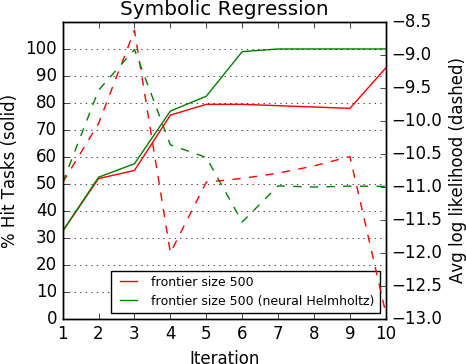
\includegraphics[width = 5cm]{symbolicRegression.png}
\end{frame}

\begin{frame}{Turtle graphics}
  Created+Investigated by Mathias Sabl\'e Meyer
  
  \vspace{0.5cm}
  
  \begin{itemize}
  \item pen up/pen down
  \item move pen (forward+rotate)
  \item get/set pen state
  \item `for' loops
  \end{itemize}

  \centering
  \includegraphics[width = 8cm]{exampleGraphicsPrograms.png}

\end{frame}
\begin{frame}{Turtle graphics}
  Created+Investigated by Mathias Sabl\'e Meyer
  
  \vspace{0.5cm}
  
  \includegraphics[width = 10cm]{turtleFigure.png}

  \end{frame}

\begin{frame}{Conclusion}

  \textbf{Takeaways:}
  \begin{itemize}
  \item Language of thought models can be engineered with fewer prior assumptions and less hand engineering
    \item Humans can flexibly adapt to new problem domains --- DreamCoder takes a step in this direction
  \end{itemize}
  \pause

  \textbf{Future work}

  \begin{itemize}
  \item A real solution to the problem of searching in the language of thought: recognition model can only go so far
    \pause
    \item Generative modeling via probabilistic programs: input/output mappings do not capture many of our concepts
    \end{itemize}

  \end{frame}

\end{document}
